%% ----------------------------------------------------------------
%% Thesis.tex -- MAIN FILE (the one that you compile with LaTeX)
%% ---------------------------------------------------------------- 

% Set up the document
\documentclass[letter, 12pt, oneside]{Thesis}  % Use the "Thesis" style, based on the ECS Thesis style by Steve Gunn
\graphicspath{Figures/}  % Location of the graphics files (set up for graphics to be in PDF format)

% Include any extra LaTeX packages required
\usepackage[square, numbers, comma, sort&compress]{natbib}  % Use the "Natbib" style for the references in the Bibliography
\usepackage{verbatim}  % Needed for the "comment" environment to make LaTeX comments
\usepackage{vector}  % Allows "\bvec{}" and "\buvec{}" for "blackboard" style bold vectors in maths
\hypersetup{urlcolor=blue, colorlinks=true}  % Colours hyperlinks in blue, but this can be distracting if there are many links.
%\usepackage{afterpage}

%% ----------------------------------------------------------------
\begin{document}

% -- blank page for library
\pagestyle{empty}  % No headers or footers for the following pages
\null\vfill
% -- blank page for library

\frontmatter      % Begin Roman style (i, ii, iii, iv...) page numbering

% Set up the Title Page
\title  {SECURE COLLECTION OF DATA IN REMOTE ENVIRONMENTS}
\authors  {\texorpdfstring
            {\href{mailto:ray@chudzinski.net}{Raymond P. Chudzinski}}
            {Raymond P. Chudzinski}
            }
\addresses  {\groupname\\\deptname\\\univname}  % Do not change this here, instead these must be set in the "Thesis.cls" file, please look through it instead
\date       {\today}
\subject    {}
\keywords   {maritime, data security, encryption}

\maketitle
%% ----------------------------------------------------------------

%% --- UHCL Approval page
\addtotoc{Signatures}  % Add the "Abstract" page entry to the Contents
\signatures
\addtocontents{toc}{\vspace{1em}}  % Add a gap in the Contents, for aesthetics

\setstretch{1.3}  % It is better to have smaller font and larger line spacing than the other way round

% Define the page headers using the FancyHdr package and set up for one-sided printing
\fancyhead{}  % Clears all page headers and footers
\rhead{\thepage}  % Sets the right side header to show the page number
\lhead{}  % Clears the left side page header

\pagestyle{fancy}  % Finally, use the "fancy" page style to implement the FancyHdr headers

%% ----------------------------------------------------------------
% Declaration Page required for the Thesis, your institution may give you a different text to place here
%\Declaration{

\addtocontents{toc}{\vspace{1em}}  % Add a gap in the Contents, for aesthetics

%I, AUTHOR NAME, declare that this thesis titled, `THESIS TITLE' and the work presented in it are my own. I confirm that:
%
%\begin{itemize} 
%\item[\tiny{$\blacksquare$}] This work was done wholly or mainly while in candidature for a research degree at this University.
% 
%\item[\tiny{$\blacksquare$}] Where any part of this thesis has previously been submitted for a degree or any other qualification at this University or any other institution, this has been clearly stated.
% 
%\item[\tiny{$\blacksquare$}] Where I have consulted the published work of others, this is always clearly attributed.
% 
%\item[\tiny{$\blacksquare$}] Where I have quoted from the work of others, the source is always given. With the exception of such quotations, this thesis is entirely my own work.
% 
%\item[\tiny{$\blacksquare$}] I have acknowledged all main sources of help.
% 
%\item[\tiny{$\blacksquare$}] Where the thesis is based on work done by myself jointly with others, I have made clear exactly what was done by others and what I have contributed myself.
%\\
%\end{itemize}
% 
% 
%Signed:\\
%\rule[1em]{25em}{0.5pt}  % This prints a line for the signature
% 
%Date:\\
%\rule[1em]{25em}{0.5pt}  % This prints a line to write the date
%}
%\clearpage  % Declaration ended, now start a new page

%% ----------------------------------------------------------------
%% - remove the quote page - chud
%% The "Funny Quote Page"
%%\pagestyle{empty}  % No headers or footers for the following pages
%
%\null\vfill
%% Now comes the "Funny Quote", written in italics
%\textit{``Write a funny quote here.''}
%
%\begin{flushright}
%%If the quote is taken from someone, their name goes here
%\end{flushright}
%
%\vfill\vfill\vfill\vfill\vfill\vfill\null
%\clearpage  % Funny Quote page ended, start a new page
%% ----------------------------------------------------------------

% The Abstract Page
\addtotoc{Abstract}  % Add the "Abstract" page entry to the Contents
\abstract{
\addtocontents{toc}{\vspace{1em}}  % Add a gap in the Contents, for aesthetics

%The Thesis Abstract is written here (and usually kept to just this page). The page is kept centered vertically so can expand into the blank space above the title too\ldots

\setstretch{2.0}  % Return the line spacing back to 2.0
Data is produced ubiquitously at sites around the globe. Many of those sites are in locations where terrestrial infrastructure such fiber optics, or copper telecommunications are impossible or, at least, impractical. The data produced is none-the-less valuable to the performance, notification and analysis of the system of this remote site. Means to collect the data over low band-width, high latency, and intermittent links exist however a key component is securing that data. To this end, we have developed a system for securing the data on the remote and queuing it until such a time as it can be transmitted. The system design and a reference implementation have been created. 

\setstretch{1.3}  % Return the line spacing back to 2.0
}

\clearpage  % Abstract ended, start a new page
%% ----------------------------------------------------------------

\setstretch{1.3}  % Reset the line-spacing to 1.3 for body text (if it has changed)

% The Acknowledgements page, for thanking everyone
\acknowledgements{
\addtocontents{toc}{\vspace{1em}}  % Add a gap in the Contents, for aesthetics

The acknowledgements and the people to thank go here, don't forget to include your project advisor\ldots

}
\clearpage  % End of the Acknowledgements
%% ----------------------------------------------------------------

\pagestyle{fancy}  %The page style headers have been "empty" all this time, now use the "fancy" headers as defined before to bring them back


%% ----------------------------------------------------------------
\lhead{\emph{Table of Contents}}  % Set the left side page header to "Contents"
\tableofcontents  % Write out the Table of Contents

%% ----------------------------------------------------------------
\lhead{\emph{List of Figures}}  % Set the left side page header to "List if Figures"
\listoffigures  % Write out the List of Figures

%% ----------------------------------------------------------------
\lhead{\emph{List of Tables}}  % Set the left side page header to "List of Tables"
\listoftables  % Write out the List of Tables

%% ----------------------------------------------------------------
%% clobber the Abbreviations - chud
%\setstretch{1.5}  % Set the line spacing to 1.5, this makes the following tables easier to read
%\clearpage  % Start a new page
%\lhead{\emph{Abbreviations}}  % Set the left side page header to "Abbreviations"
%\listofsymbols{ll}  % Include a list of Abbreviations (a table of two columns)
%{
%% \textbf{Acronym} & \textbf{W}hat (it) \textbf{S}tands \textbf{F}or \\
%\textbf{LAH} & \textbf{L}ist \textbf{A}bbreviations \textbf{H}ere \\
%
%}

%% ----------------------------------------------------------------
%% clobber the llist of constants - chud
%\clearpage  % Start a new page
%\lhead{\emph{Physical Constants}}  % Set the left side page header to "Physical Constants"
%\listofconstants{lrcl}  % Include a list of Physical Constants (a four column table)
%{
%% Constant Name & Symbol & = & Constant Value (with units) \\
%Speed of Light & $c$ & $=$ & $2.997\ 924\ 58\times10^{8}\ \mbox{ms}^{-\mbox{s}}$ (exact)\\
%
%}

%% ----------------------------------------------------------------
%% clobber the symbols - chud
%\clearpage  %Start a new page
%\lhead{\emph{Symbols}}  % Set the left side page header to "Symbols"
%\listofnomenclature{lll}  % Include a list of Symbols (a three column table)
%%{
%% symbol & name & unit \\
%$a$ & distance & m \\
%$P$ & power & W (Js$^{-1}$) \\
%& & \\ % Gap to separate the Roman symbols from the Greek
%$\omega$ & angular frequency & rads$^{-1}$ \\
%}
%% ----------------------------------------------------------------
% End of the pre-able, contents and lists of things
% Begin the Dedication page

%\setstretch{1.3}  % Return the line spacing back to 1.3
\setstretch{2.0}  % Return the line spacing back to 2.0

\pagestyle{empty}  % Page style needs to be empty for this page
\dedicatory{For Nicholas, Anastazja, Katy and all my family for their continuous patience and support\ldots}

\addtocontents{toc}{\vspace{2em}}  % Add a gap in the Contents, for aesthetics


%% ----------------------------------------------------------------
\mainmatter	  % Begin normal, numeric (1,2,3...) page numbering
\pagestyle{fancy}  % Return the page headers back to the "fancy" style

% Include the chapters of the thesis, as separate files
% Just uncomment the lines as you write the chapters

\lhead{\emph{Introduction}}
\chapter{Introduction}
Remote communications have become the backbone for industries at sea. The energy and shipping industries remote sites are, in the case of fixed position vessels, are remote or, in the case of ships at sea, traveling long distances. The communication infrastructure used by these remotes has the defining characteristics of low bandwidth, high latency, and intermittent connectivity. Under these conditions, there is demand for secure capture and transmission of information.\cite{Levinson:2010wm} This project serves to present a system, which can securely deliver that data. 
This paper presents a high level overview of the system; it’s architecture, the component systems, and a reference implementation. Upon that, a threat analysis is used as a benchmark. Several attacks are employed using both classical and modern techniques as of this writing.
The research presented here are intended to address a problem in securing that information. The benefits to this research are to make this data available for analysis and mitigate the potential for loss. We do this by describing methods to capture and, securely transmit the data. Securing the information assures that it is free from corruption, unauthorized access and from a confirmed origin.
 % Introduction

\lhead{\emph{Problem Definition}}
\chapter{Problem Definition} 
\section{Motivation and Sample Applications}
The wide geography covered by the vessels requires global coverage. Because of this few assumptions can be made about the network link from region to region. 
The problem of remote data security exists in many use case applications. In this paper we reference example applications involving maritime shipping, and maritime energy production. Maritime, as it refers to shipping, has challenges regarding the tracking and monitoring of cargo. Worldwide, there are in excess of seventeen million shipping containers.\cite{Levinson:2010wm} They are used to transport perishable cargo or raw materials otherwise sensitive to environmental attributes such as temperature, humidity, vibration or tilt. 
A specific example might be a shipping of New England tuna bound for Japan. In this case, proposed shipping requirements in the fishing industry require that the temperature must strictly maintain a temperature of -40° C to –45° C during transit. A solution must allow for logging values and, alarming for environment thresholds (temperature, humidity), and security (doors opened in transit) in those containers. need to be stored until a transmission path becomes available.
Petroleum Energy production has seen a drastic increase in production since in recent years as the price of crude has stabilized at historic highs.\cite{Anonymous:ko4JQlUG} Drilling efforts are moving into more complex environments, such as offshore drilling, and deep water drilling in the Gulf of Mexico. By virtue of the terrain surrounding deep-water environments, terrestrial communications infrastructure is not available. The most common solution is a satellite connection. Operating details such as those from the drill, pumps, storage tanks and real-time activities require continuous data communications with systems on shore. A specific case can be drawn from the explosion aboard the Drill Ship Deepwater Horizon. After the explosion on April 20th 2010, a preservation of evidence order \cite{Fenton:2011kq}was announced. Our system can potentially create and maintain security of that collected evidence and this can be done even before a triggering event occurs (e.g., data collected immediately before the explosion). In the Gulf of Mexico there are 2400 drilling rigs of which two-dozen are operating in deep water\cite{Anonymous:ko4JQlUG}. The potential need for secure information has become a necessity. To be secured, the properties authentication, availability, confidentiality and origin integrity.)
Tracking of air pollution data at relay stations where the security of such data must follow a chain of ownership.  The evidence gathered in a crime scene where a chain of customer must be maintained.\cite{Group:2006en}  The processing of event data in a drilling site where timestamps and irrefutably are crucial for investigation when that remote may no longer have the data stored on the remote. 

\section{Related Work}
Palsberg et al, \cite{Palsberg:1997ts} discuss an end to end solution for transmission of messages. The solution they present does inform our decisions however it lacks a provision for handling situations when the transmission link is unavailable. We address this through the design of a store-and-forward solution.
Schneier \cite{Schneier:1999fu} proposes a method for securing log entries. The solution requires the use of a trusted third party. We address this with a pre-shared, out-of-band distribution of certificates.
A useful work from Mumar and Handzinski\cite{Kumar:2012vg} provides details on how RESTful protocols can be applied. We reference this in the implementation as background for are use of REST.
\section{Assumptions}
This solution assumes that the physical access to the remote device is controlled and the data inputs are properly managed. Specifically, the collection devices and their inputs outside of the system are considered to be secure. For the system these devices and inputs are taken to be the ingress point for raw data. It is at this point that we consider the information secure. The data from here is passed via messages that are defined below. Equally, the processing and storage hardware at the data center is secured assumed to be physically secure. Access to persistent storage (hard disk or SSD), memory, or the network interface adapter, is a significant vulnerability and outside of the scope of this investigation. 
The keys used in the communications are provided to the remote device in a secure manner before installation. The presence of this pre-existing key agreement is delivered out-of-band of the network path used by the messaging and loaded onto the node at install time. 
The sites’ inability to rely on high bandwidth, low latency associated with terrestrial communication links provides challenges. Our system assumes and addresses the need to secure the data while the data center server is unavailable. During the periods in which communications are not available, the nodes will secure and store the messages until connectivity is resumed.
     The use of the term security in this paper is used with respect to confidentiality, integrity, availability, authenticity, and non-repudiation. These security properties and maintained throughout the system.
     
\section{Information Security Attributes Definitions}
Security and the properties of security are listed here for clarity. These definitions represent the terms usages in the paper.
\subsection{Integrity}
The integrity in our system refers to "\ldots the trustworthiness of data or resources."
\cite{Bishop:2003ug} Integrity prevents the undetected change to the data of a message. Message integrity applies to the message, both when it is being transmitted over the network (‘in-flight’)  as well as when it is stored on persistent storage and when it is in memory.\cite{Levinson:2010wm}
\subsection{Confidentiality}
Confidentiality is the property that prevents unauthorized users from being able to read the message. Encrypting the data portion of the message with a high-entropy key and secure algorithm creates a message that an observer cannot decipher. The system must maintain confidentiality of the messages through the system including when stored. We provide this using multiple mechanisms in the message’s lifecycle. 
\subsection{Authentication (Origin Integrity)}
Origin Integrity is the property whereas a sender cannot be impersonated. todo 


[There exist different types of ‘origin integrity’: creator OI, signer OI, sender OI, etc. Are you planning on dealing with all of them?]


\subsection{Availability} 
Availability is the most critical concern of this system. As messages are generated onboard the remote site, critical data is being created. Each message, representative of an event, is part of the overall status of that site. In our problem we focus on the assumption that the backhaul to the data center is intermittent. In order to ensure the availability of the data we secure store the messages until the backhaul returns and connectivity is reestablished. Availability, in this strict sense, is the presence of the messages to be transmitted.
\subsection{Non-Repudiation}
Non-repudiation is the … “security service by which the entities involved in a communication cannot deny having participated.”\cite{Kissel:2013vu} In our particular case we assert that a message having been sent cannot be denied by the sender. This is of great importance in our solution. Use cases where the messages leading up to an event must be veritably sent from a known sender (or senders). The two components of non-repudiation are message integrity and origin integrity (authentication).  Message integrity is provided using the hash message authentication code (HMAC). Origin integrity is provided using a digital signature. 

 % Problem Definition

\lhead{\emph{System Design}}
\chapter{System Design}

\section{System Components}
In this chapter we will provide an overview \autoref{fig:systemComponents} of the components of the system and their function. The overall system is divided into three components remote data collection, data transport and, the server processing and storage.  It is presumed that the remotes have varying locations (although they may stay in a single place for months or years). Remotes are not specifically tied to any geography.  They may be it marine or land based. In this discussion, examples are assumed to be a marine application.  

\begin{figure}
\centering
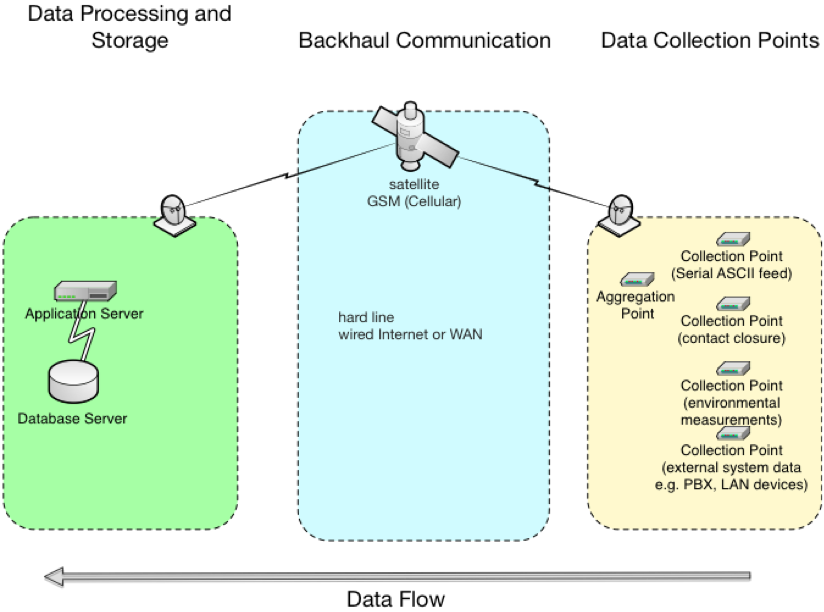
\includegraphics{Figures/systemComponentOverview}
\caption{System Components}
\label{fig:systemComponents}
\end{figure}
\section{Data Collection Component}

The layout of the data collection component tiered and resides fully on the remote site.  The devices that act as collection points are known in our system as nodes.  They are installed on-board with the tasks to receive, secure and transmit the data.  A remote site must house at least one node but may have multiple nodes installed.  Each node, in turn, is comprised of one or more data inputs called tendrils.  A tendril is a single source of data which reports directly to the node. 

\subsection{Nodes}

The node uses a small on-board device which is capable of running a general use operating system. For our mock up node, a BeagleBoard\cite{Anonymous:zgMDnVpL} brand embedded device is used.  The node is designed to have a small resource footprint with CPU, memory and storage capacity restricted and cost effective.  The device is configured with 512M of RAM, a single code CPU, and 1 Gig of SSD disk storage.  The CPU draws very little power and produces minimal heat.  This relieves a requirement for a fan in most applications and results in a device with no moving parts.  

A node may receive inputs from a variety of sources.  Each node's id is unique throughout the system.  With a unique id it is possible to have many nodes installed on a single remote site and across sites and nodes can be migrated to other sites. This proves useful in the case that a datasource is moved. For instance if a cargo container is transported to another ship. 
In our reference implementation we will limit to a single node with multiple simulated inputs.  These inputs are referred to as tendrils that are tasked to provide the events to the node.  The node will accept to a variety of different tendrils and collect their event information.  

\begin{figure}
    \centering
    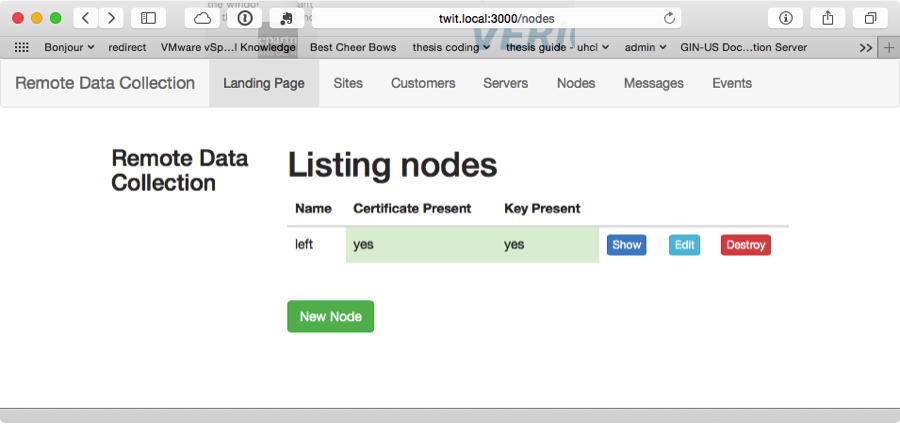
\includegraphics[scale=.9, angle=0]{Figures/interfaceNodes}
    \caption[Nodes Interface]{Web Based Interface for Node Management}
    \label{fig:interfaceNodes}
\end{figure}

\subsection{Tendrils}
The idea of the tendril is one of flexibility. 
It is designed with an abstraction layer based on the REST protocol. A wide variety of information is made possible by this design. 
Example types include Environmental, State Change Detection, Location, and events sent by intelligent systems.  
More specific examples include: ambient temperature, humidity, door openings and closures of a cargo container, GPS position, wave height, wind speed and sophisticated system activities such as phone calls and email activity. We create three types of tendril inputs although any number may be possible. Contact closure, serially attached streams, and intelligent system messages present an overview of what is possible. 
\subsubsection{Contact Closure}
Contact closures\cite{OmegaEngineeringInc:vi} in this context would have a circuit connected to a relay on a door, for example. Opening the door also creates an open circuit is detected by our agent. The event is recorded and secured on the agent with a timestamp and position if available. The purpose of such a measurement is to detect a container being accessed. The event, once processed, is compared against a policy of access that determines if the access was authorized. The converse of this is to detect events that are scheduled to occur. For example detection of a fuel cap being removed on a generator to indicate it was inspected. \autoref{fig:contactClosure} Contact closure relays are low cost devices that can be configured as a tendril\cite{Anonymous:wa}.
\begin{figure}
\centering
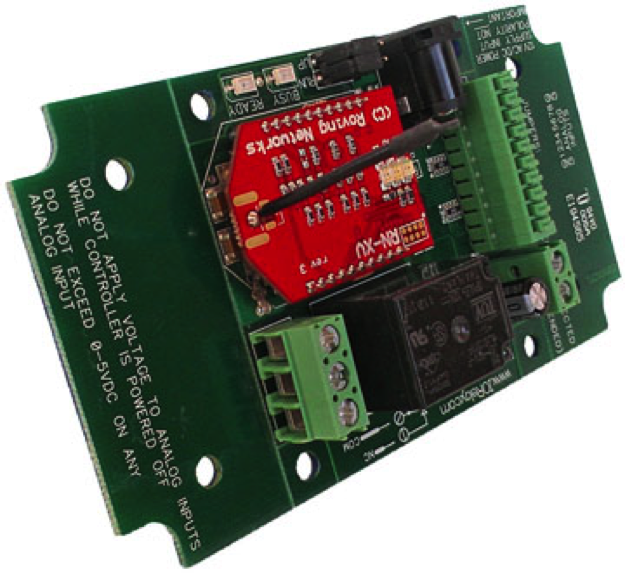
\includegraphics{Figures/contactClosure}
%\caption{Contact Closure - RelayPros R110PL_WIFI WiFi Relay}
\caption{Contact Closure - RelayPros Wifi Relay}
\label{fig:contactClosure}
\end{figure}
\subsubsection{Serially Attached Systems} 
Serially attached systems are considered to be systems attached via an RS–232 or similar pinned connection. They are devices that have a serial console connect which provides either a stream of character data or an updated status screen. An example is a GPS device which provides a NEMA string. A device in this configuration has a consistent stream of ASCII data using a standard protocol. GPS positioning coordinates as well alarms and electronic fence data are sent down the serial link to the attached node. Within the node, as with all devices, the stream data is secured in messages for transmission to the storage systems.
\subsubsection{Intelligent Systems}
We recognize a third category of tendril data sources termed intelligent systems. They have the ability to process, compile and digest their information before collection. They have significant processing power and can transmit over a local network to the local node.  
Examples of these are VoIP call managers, routing, switching, and WiFi infrastructure, and servers.  These can record call detail records for from call managers, routers and infrastructure log data, and diver / ROV  \cite{Christ:2011vn} video systems.
Potential use cases include but are certainly not limited to: Logging Environmental Systems Call Manager Systems, Email, and Cell phone usage
The end result of all this information collection with the remote is the standard interface that feeds the message. Upon. The remote upon receiving an input it will take me information contained and security and the message Block. These message locks are then either transferred immediately or stored and transferred once the system is online.
During the Deepwater Horizon explosion, many elements of data were generated leading up to the explosion itself. 
Much of this data was from the phone system and cellular network. Both of these could have been captured and transmitted up to the point that connectivity was lost. 


\section{Transmission}
The transmission component of the system, also referred to as the backhaul, can be provided by a number of network topologies and technologies. Therefore we can make few assumptions about it’s quality, bandwidth, or availability. The system therefore treats the transmission component as a generic pipe. The one assumption that we do make is that the connection must be available before the node resources are exhausted. This will vary depending on the application but generically we expect communication to be resumed available every 24 to 48 hours. Practical expectation is that connectivity would be more frequent and stable.

This backhaul link is also assumed to be inherently insecure. Public networks such as the Internet and cellular phone networks will be routinely used. Therefore all security is managed within the message block itself. Key exchange (key agreement) is provided using a pre-shared, symmetric key. In this model the message processing does not require the transmission link to be online when messages session key is created.

\section{Storage and Processing}
The storage and processing component of the system is the server that lives within the data center. The site would be a corporate installation owned and controlled by the end user. Security of the physical system and access to the operating system are assumed.  Messages received by the server are decrypted and placed into the database. Depending on the sensitivity of the message appropriate database level encryption can be used for increased protection and prevents access by an authorized user should the system be breached. 

The storage and processing component of the system is composed of three functional pieces. At its base provides a data store for the messages to be decrypted and stored. and available for processing. Secondly, it provides the business logic interface for configured rules and their thresholds. Finally it is the user interface for provisioning and management, and key management the node devices. 

\section{Reporting}
As part of the storage and processing we expect to produce a geographic mapping application \autoref{fig:interfaceMap} to show the position of the nodes as they traverse the. 
Popup values such as online / off-line, number of messages received, and time since last contact. The interface should also provide the ability for the user to correlate events. E.g. correlate by time, by a fleet, by system type. 

\begin{figure}
\centering
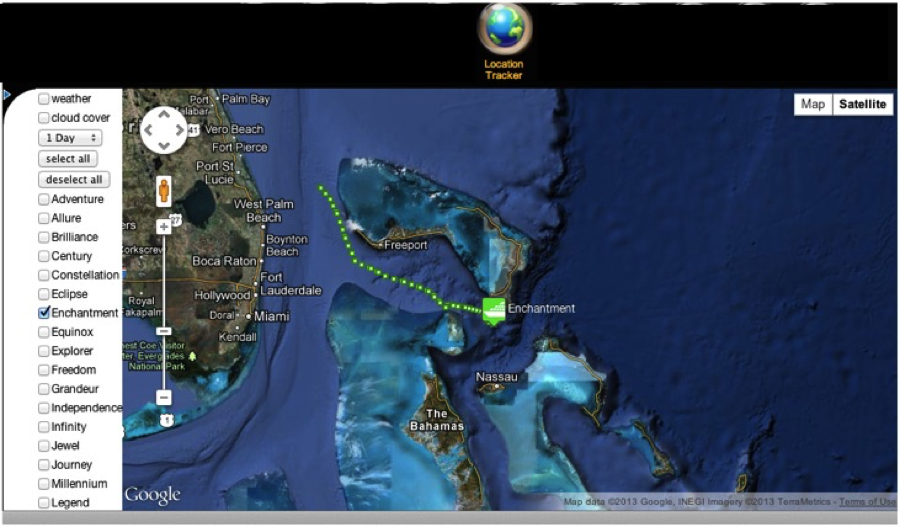
\includegraphics[scale=.9]{Figures/interfaceMap}
\caption{Map Interface}
\label{fig:interfaceMap}
\end{figure}

\section{Messages}
Requirements for our solution are securing the information at the time of collection, transmitting the information securely and, storing the information in the data center securely. To address these we have designed message formats and protocols to mitigate the threats. Our solution provides the following security attributes:  confidentiality, integrity, and non-repudiation (authentication). 

The message format is composed of the payload, and a hash message authentication code (HMAC). For the event data we look inside the payload. It contains the timestamp, ids for both the tendril and the node, and the event data itself. The event carries two fields within it didn’t type and it’s content.  To manage the data on the remote we designed process that begins with an input at the tendril. The element manager through either polling or an event will signal the node to create a message. The node then takes this event data and formats it into a message. The message format contains a hash of the payload (HMAC), which provides data integrity. (detailed below) Encryption with a shared key provides the confidentiality. Our process of key management, which is discussed below, handles origin integrity, nonrepudiation or authentication.   Once even has been processed into a message and secure, it is handed off to the transition component where it will either be transmitted immediately or store on the remote node.

\subsection{Digital Signature Algorithm}
The format supports the integrity property by default. As mentioned above, Integrity is maintained by use of a message authentication code (MAC) on the payload data. A hashed MAC (HMAC) employing SHA-2 is chosen in order to avoid known hash collision exploits found in other hashing algorithms. \cite{Turner:MiRyW-r_} 

\subsection{Encryption Algorithm}
Encryption is centered on the public/private key pair created and stored at install time of the node. A 1024k bit RSA algorithm is used to generate both a server and a node key pair. 

The shared key is used to generate a message specific key that in turn is used to encrypt the payload of the message. The server side of the system uses the same shared key to generate the message key. This provides the benefit of the shared key never being transmitted on the network. This property of key hiding is a key feature in defending against eavesdropping based attacks.

\subsection{Certificate and Key Management}
Certificates and Keys are required to provide confidentiality, origin integrity and destination integrity. Server certificates are loaded into the remote nodes at provisioning time and conversely the server generates and stores a certificate for each node in the network. The system uses two types of certificates, the root Certificate Authority (CA) certificate and the endpoint certificate. 
The CA is a root certificate used to sign all certificates, endpoint certificates as well as itself. The endpoint certificates hold the information required to authenticate the sender, and support encryption. The CA provides a chain of authority that each endpoint certificate is unique. 
Certificates provide proof of server identity to each node and the presence of the client side certificate on the node allows the server to identity the individual node (sender authentication). 
The manner in which the certificates are distributed to the server and remotes protects us from imposter attacks on both sides of the transmission. This is discussed further in the threat analysis section. 
  The public keys embedded in the certificates are used to authenticate the server and remote to each other. 

\subsection{Message Handling}
  Messages are secured as the node generates them. We ensure message integrity, authentication, confidentiality and availability through the following steps. (non-reputability, origin integrity, and sender integrity provided during the transfer phase.) 

  1.  The node detects an event on a connected tendril.
  2.  A message is created from the event with the event properties. (see Figure ‘Interface Events’ )
  3.  The message and the node’s private key ( $k_{pub}$ ) is used to create a digital signature.
  4.  The message and the digital signature are concatenated to form $m_{signed}$ .
  5.  $m_{signed}$ is encrypted with the server’s public key to produce $E$ .
  6.  $E$  is stored to the node’s local storage.
   
   Figure 4.3 - Interface Events
\subsection{Message Components}
   Nodes use the transmission link to send data messages to the server. The most efficient means of communication is when the remote has a direct connection to the server. Direct connect is characterized as a state where the node can open a TCP socket to the server. Having a direct connection, confidentiality, integrity and non-repudiation are provided via a combination of SSL/TLS, HMAC, and Digital Certificate that we detail below.
    
    Figure 4.4 - Interface Messages
In the case that the connection to the data center is not available or intermittent / degraded connectivity places the system in ‘store and forward’ mode. 
When the link is down the messages are stored on the node in a FIFO message queue (there their signed and encrypted format). As many messages are held as possible. The number that can be held in memory is dependent open two resources, the amount of storage and the amount of RAM on the node.
Encryption is required on all message transmission to and from the nodes. The node use symmetric, shared key encryption protocols to reduce processing resource requirements and minimize time spent handling messages. 

\section{System Initialization}
    As part of the project client-side and server-side certificate key management are investigated as well as various key exchange and data channel encryption methods. Threats to the security of the system are key to this design. The defenses against those threats are analyzed below.
\subsection{INITIALIZATION OF REMOTES}
    The server and remotes are initialized at deployment time. This is when the remotes are given unique identifiers and credentials for interacting with the storage server. Conversely, the server stores the information required to identify each remote.  
    Key Distribution
    Key distribution at system initialization is performed out-of-band. Meaning we do not transmit the keys over the production network. Remotes are intended to be physically accessible and the pre-shared interchange key, which has been generated by the server, is installed onto the remote directly.
\subsection{OPERATIONAL SYSTEM KEY MANAGEMENT}
     
     Figure 4.5 - Interface Certificate Management

\section{Transfer Protocol}
     In order to transmit the message from the remote to the server, a socket-based protocol is needed. For this we chose to use HTTP for its simplicity wide usage and clear protocol definition. \cite{Moore:we, Fielding:eSmSU8EF} 
     HTTP also has the advantage of providing TLS/SSL encryption and seamless integration with certificate libraries. We make use of TLS/SSL to provide security when the messages are sent. 
     On top of HTTP we employ the REST (REpresentative State Transfer) protocol. \cite{Fielding:2000dd}  In brief REST allows us to use the standard HTTP subcommands or ‘verbs’ ‘GET’, ‘POST, ‘PUT’, ‘PATCH’ and ‘DELETE’ to manipulate elements of the system and treat all those elements as resources. 
\subsection{REST AS A SUBSTRATE}
     As a brief introduction to REST it helps to point out the pieces of the HTTP protocol of specific interest. We also lightly cover the relationship between REST over HTTP, and our use of TLS/SSL.   
     The Transport Layer Security / Secure Socket Layer is a security layer protocol “… used for encapsulation of various higher level protocols.”{dierks:wd}  In our case  we use TLS to secure out HTTP connections. \cite{Rescorla:2000tv}.  This provides, confidentiality, integrity and authentication for our messages during transmission. 
     The REST protocol, now secured via TLS, incorporates the concept of a resource and actions upon those resources. REST provides four actions we will use.  Those are ‘Create’, ‘Read’, ‘Update’, and ‘Delete’.  
     Create, Read, Update and, Delete.  
     “The World Wide Web, where HTTP [5] is the uniform interface. HTTP defines the verbs GET, PUT, DELETE, POST, PATCH [4], OPTIONS and HEAD.” 
      The REST methods are mapped to a corresponding HTTP verb.  \cite{Fielding:2000dd}
      REST Method HTTP Verb Safe / Idempotent
      Create  POST  Idempotent
      Read  GET Safe and Idempotent
      Update  PUT Idempotent
      Delete  DELETE  Idempotent



\subsubsection{Safe and Idempotent}
      REST and the HTTP verbs used in this system participate in two properties. The methods apply to some methods but not others.  The property ‘Safe’ ensures that the action provides a resource in response and the action must not have any side effects. This also means that the action, when applied to the resource, leaves the resource in as the same state as it was in before the action.  Multiple read calls using will return same resource state.  
      The Idempotent property of an action guarantees that a resource will end in the same state over multiple calls. For example, calling ‘create’ on a single resource results on only one instance of the resource being create.  Just as calling update multiple times on a given resource with the same attributes will result in the resource being set to the same state as calling the action once.  The HTTP ‘GET’ verb is of particular importance as it is the only action that is both ‘safe’ and ‘idempotent’.  
      The state of the resource (and all other resources) must be the same before and after the method call.  ‘Create’, ‘Update, and ‘Delete’ are called with the intention of modifying a resource and are considered ‘Idempotent’.  Similarly they are not considered ‘safe’.  It is assumed by the client that the state can change.  
       Values are passed in the request for ‘create’, ‘update’ and ‘delete’ actions.  They are typically passed initial values such as a name and its relation to other resources or in the case of a delete, an identifying attribute.  REST uses the HTTP verb ‘POST’ to create new resources.  
       Example REST routes
        
        Figure 4.6 - REST routes and actions for the node resource
\subsection{JSON}
        The REST methods defined the action on a resource, however we need to be able to pass attributes to the resource. To this end we selected JSON (JavaScript Object Notation){Bray:1aMFfDtC} JSON has the benefits of being human readable and well supported. Many libraries and languages exist to parse it. In our case, the Ruby libraries we use are conveniently built into our basic client / server install.  





 % System Design

\lhead{\emph{Securing the Data}}
\chapter{Securing the Data}
The system is designed with one overarching goal. That is to securely capture the remote data and preserve it for later use. For this we have designed a message format that is secure during both collection and transmission. The message data and the event data are carried in the message payload. \autoref{fig:messageDatagram} 
Collecting and storing the data have different security requirements and we treat each with a separate security mechanism. 
During the lifetime of a message, \autoref{fig:messageLifetimeOverviewDiagram} it is created on the node and stored, and later transmitted. While the message is in the stored state, message security properties are confidentiality, integrity, and availability. We refer to this stored state as Message Security. When the system is ready to send, the tasks required to support authentication (both sender integrity and recipient integrity), confidentiality data integrity, and non-repudiation are managed. We refer to this step as Transmission Security.
\begin{figure}
\centering
\includegraphics[scale=.75]{Figures/"message datagram"}
\caption{message datagram}
\label{fig:messageDatagram}
\end{figure}

\begin{figure}
\centering
\includegraphics{Figures/"message lifetime overview diagram"}
\caption{message lifetime overview diagram}
\label{fig:messageLifetimeOverviewDiagram}
\end{figure}

\section{Transmission}
Securing the transmission is divided into two phases. The first phase provides authentication. The outcome of the first phase is the production of a session key. The second phase is the secure transmission of the data confidentially. 
We make use for TLS / SSL for the transmission. TLS / SSL a standarized protocol which will be familar to most readers as it is most often used in securing HTTP. (Browsers reference secured resources with the https protocol identifier.) HTTPS in the browser is, again, most often used to authenticate a server to a browser. This type one way authentication can be augmented with client side authentication. Authentication of both the client and the server is known as mutual authentication.  

\subsection{Certificate Mutual Authentication}
\subsubsection{Phase 1}
In phase one we use x.509 certificates as a means of authenticating the origin of the data.
The certificates required are the ones installed at system provisioning ( $A{_{cert}}$ and $B{_{cert}}$ ). 
The server and the node can trust the certificates to be correct and authentic. The trustworthiness is based on two factors. 
\begin{itemize}
\item The certificates were installed out-of-band of the data and 
\item each server and node has a certificate for the other. 
\end{itemize}
Given that we trust our certificates and that the server and node have each other’s respectively, we can mutual authentication. 
Mutual authentication means that not only does the node know the identity of the server but also the server is confident of the nodes identity. 
Below is a list of steps for mutual authentication diagrammed in \autoref{fig:mutualAuthenticationMessages}:

\begin{enumerate}
\item The node initiates a transmission with a certificate request to the server. 
\item The server responds by sending its certificate. \\ $A{_{cert}}$ \par
\item The server responds with a certificate request for the node and a plaintext message. $m$
\item The node calculates a cyphertext message $m$ encrypted with the nodes private key to produce cyphertext. \\
$c=E{_B{_{priv}}}$
\item The node sends its own certificate $B{_{cert}}$  to the server concatenated with the cyphertext.  \\$B{_{cert}} + c$
\item The server uses the node’s public key, $B{_{pub}}$ , to decrypt the cyphertext and produce its own copy of message $m'$\\$m'=D{_B{_{pub}}}(c)$
\item The server compares $m′$ with the message $m$ that it had sent previously. If $m'$ is equal to $m$ the session moves on to RSA key agreement. \\ $if (m == m')$
\item The key agreement negotiation results in a session key. $k{_session}$ 
\end{enumerate}
 
\begin{figure}
    \centering
    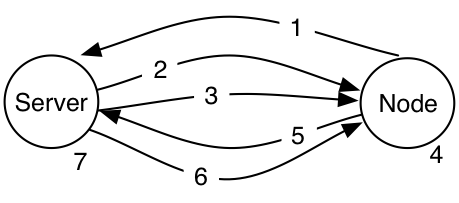
\includegraphics[scale=1, angle=0]{Figures/mutualAuthenticationMessages}
    \caption[Mutual Authentication Messages]{Mutual Authentication Messages}
    \label{fig:mutualAuthenticationMessages}
\end{figure}

The outcome of this first phase is the production of a session key. Using certificates, a chain of trust is established which is used to provide origin integrity for an asymmetric (public/private) key pair. 
These asymmetric keys contained in the certificates are used to verify the identity of the opposite end of the connection and then, once identity has been confirmed, those keys are used in key agreement to establish a session key. 
\cite{Rescorla:2000tv}, \cite{Viega:2002wt}, \cite{Oppliger:2014wm}

\subsection{Secure Communication}
\subsubsection{Phase 2}
The symmetric session key from phase one is now used as a ‘master session key’ from which each transaction will derive an individual key. The use of session keys provides confidentially during transmission. The master key is used to create session keys which also affords us forward secrecy.  

\subsection{Message Security}
The first step in securiting the messsage is securing the payload. 
At this point, the security properties of confidentiality, integrity, and availability are provided.

\section{Message Lifecycle}
The message is instantiated upon the arrival of an event from the node’s input tendril.  The event is recorded in the message payload and a message authentication code (MAC) is applied. The resulting data and MAC are concatenated to produce a record (rx).  \\
$data + MAC = r{_n}$
 
A corresponding symmetric record key, $k{_n}$ is created and used to encrypt the record. Each key is specific to the message. Each message as one key and each key belongs to a single message. The encryption uses this $k{_n}$.  symmetric key generated by the node.  The encryption yields cyphertext $c{_n}$ .  
Confidentiality is provided by the use of encryption while the message is stored. \\
$E{_k{_n}}(r{_n}) = c{_n}$ 

Once encrypted record $c{_n}$ is saved to storage on the node.  

Message records are created by a triggering event may occur at any time. Due to the assumption that we have intermittent communications, availability requires additional handling. Ensuring availability requires that messages be preserved on the remote until they can be transmitted to the data center server. As we show in the section above, the messages are encrypted and stored at the time of instantiation.  When the connection to the data center server becomes available, the messages are transferred. 
% replaced with vector pdf named messageLifetimeOverviewDiagram
%\begin{figure}
%    \centering
%    \includegraphics[scale=.9, angle=0]{Figures/messageLifecycle}
%    \caption[Message Lifecycle]{Message Lifecycle}
%    \label{fig:messageLifecycle}
%\end{figure}
 % Securing the Data

%\input{Chapters/Chapter2} % Background Theory 
%
%\input{Chapters/Chapter3} % Experimental Setup
%
%
%\input{Chapters/Chapter5} % Experiment 2
%
%\input{Chapters/Chapter6} % Results and Discussion
%
%\input{Chapters/Chapter7} % Conclusion

%% ----------------------------------------------------------------
% Now begin the Appendices, including them as separate files

\addtocontents{toc}{\vspace{2em}} % Add a gap in the Contents, for aesthetics

\appendix % Cue to tell LaTeX that the following 'chapters' are Appendices

\lhead{\emph{Implementation Details}}
\chapter{Implementation Details} The implementation of the system is one of the work products that we targeted. To describe the construction we divided the implementation into the layers of logic, and where it applies in the system.  The model is represented on the node, during transmission, on the server, or in reporting.  
At its base there is an object model that is used in both in memory and on disk.  The object model provides a consistent and organized view of all the configuration items and data items. For instance a node is a physical device that is deployed on a remote. When provisioned the node is added to the database as a configuration item{Bernard:2012vp}. The node is also initialized with the information unique to that node such as its id and the id of the server.  The database will them record a copy with additional attributes such as the date of creation of the node and its configuration.
During transmission we focus on the message object. The message is the model that gets transmitted between systems.  Messages are transmitted using a webservice from the node to the server as the backhaul permits and are seamlessly captured and stored by the server. 
Finally, on the server, we have processing, storing, and reporting functions that rely on the full model structure.  The configuration item data that stored during provisioning is matched against the data encrypted in the message. If the message is valid, it can be assumed that it has maintained confidentiality, integrity and authenticity. 

\section{Object Model}
The object model is designed to reflect the physical elements and relationships between objects. Instances of the objects are held in the memory and on the network as well as in storage. To allow for a logically seamless integration, we employ an Object Relational Mapper (ORM).
This abstracts the persistence of the object using the ActiveRecord ORM pattern \cite{Fowler:2012wd} and fits well with the REST webservice.  Each class in the object model roughly corresponds to a RDBS table or set of tables. The ORM allows for flexibility in design for future implementations of the storage layer.

\subsection{Nodes}
The fundamental object is the node. \autoref{fig:logicalModelNodes} It is a physical object that is also represented in the database.  Its configuration contains the encryption keys, X.509 certificates, and collection algorithms on the remote.  In our implementation the node is a low-power device that has connectivity to the backhaul (and then virtualized for testing).  The node is responsible for transmitting, queuing, securing, and collecting the event and message data.  
\begin{figure}
\centering
\includegraphics[scale=.9]{Figures/"logical model diagram - node highlight"}
\caption{logical model diagram - nodes}
\label{fig:logicalModelNodes}
\end{figure}

\subsection{Tendrils}
Attached to the nodes are tendrils. Tendril is our term for the data source being presented.  Tendrils handle inputs from a range of services. For example, a node can receive ASCII streams of data over TCP/IP, or over serial, or contact closure connections. The other major input type is SNMP (Simple Network Management Protocol) and UPnP message events such as temperature alarms from a network device. 

\subsection{Messages And Events}
\autoref{fig:logicalModelMessagesAndEvents}
 \begin{figure}
 \centering
 \includegraphics[scale=.7]{Figures/"logical model diagram - messages and events"}
 \caption{logical model diagram - messages and events}
 \label{fig:logicalModelMessagesAndEvents}
 \end{figure}

\subsection{Customers and Sites}
The term site refers to the physical location where a node or server is present. A remote site typically is a ship or an energy production vessel. They may change location continuously (as in the case of a ship) or be moored to a single location for months, like a production petroleum rig.  Site has a special consideration when it comes to position attributes (latitude and longitude).  Position can be considered one of many attributes delivered by the message.  However, do to the map reporting tool we extract position as the messages arrive.  To round out the object model we have a customer object with names and personnel details.
\begin{figure}
\centering
\includegraphics[scale=.8]{Figures/"logical model diagram - customers and sites"}
\caption{logical model diagram - customers and sites}
\label{fig:logicalModelCustomersAndSites}
\end{figure}
 
Appendix Figure 3	Object Model – Customers and Sites	

\subsection{Server}
The server is the destination for all of the data.  It is designed to be in a datacenter or in a shorebase.  It keeps a catalog of all the keys and certificates assigned to nodes. As each node is provisioned, an X.509 certificate and a key is generated and stored on both the server and the node.  The server contains the CA certificate for the system. It is used for signing all of the node certificates.  
\begin{figure}
\centering
\includegraphics[scale=.7]{Figures/"logical model diagram - server"}
\caption{logical model diagram - server}
\label{fig:logicalModelServers}
\end{figure}
Appendix Figure 4	Object Model Server

\section{TLS / SSL Tool}
\subsection{Installing OpenSSL}
The TLS/SSL solution used is openssl\cite{Anonymous:DuAhrSbO}.  It has a deep feature set including current encryption and hashing algorithms.  
The first step in building the system is to install the openssl development command line application and its libraries. This will also ensure that the dependencies are installed. On the Centos Linux system the ‘yum’ tool is used.  From the command line and as super-user ‘root’ run the following from the command line. \par

\begin{lstlisting}
yum install –y libyaml-devel, autoconf, gcc-c++,\
 readline-devel, zlib-devel, libffi-devel,\
 openssl-devel, automake, libtool, bison, sqlite-devel 
\end{lstlisting}
\par
%\newpage
Once this completes you can verify the installation. 
\begin{lstlisting}
[root@host root]# openssl
OpenSSL> version
OpenSSL 1.0.1e-fips 11 Feb 2013
OpenSSL> 
\end{lstlisting}

OpenSSL version 1.0.1e is the latest at the time of this writing, however, any install should use the latest version generally available.  

	% Implementation Details
\chapter{Glossary}
\textbf{CRUD}        \textbf{C}reate, \textbf{R}ead, \textbf{U}pdate and, \textbf{D}elete – A collection of resource functions to manage RESTful resources for managing resources. They roughly correspond to the SQL actions of Insert, Select, Update, and Delete, respectively.

\textbf{Datacenter}      A physical location housing the primary servers and network infrastructure.

\textbf{Fleet}      a group of sites belonging to a single entity (e.g. all of the vessels owned  by Acme Corp)

\textbf{NEMA}        

\textbf{Node}– A device on the remote that collects the event data and creates messages. The node is responsible for holding the messages until such time as they can be transmitted to the server.

\textbf{Out-of-band}– The transfer of information outside of the common communication channel or network.

\textbf{GUI}– Graphical User Interface

\textbf{In-flight}- Information that is in the state of being transferred.

\textbf{JSON}– Javascript Object Notation

\textbf{REST}– \textbf{RE}presentative \textbf{S}tate \textbf{T}ransition – This is the protocol that provides the web services used between the node and the server.{Fielding:2000dd}

\textbf{ROV} – \textbf{R}emotely \textbf{O}perated \textbf{V}ehicle. A remotely operated submarine for the context of this paper.{Christ:2011vn}

\textbf{SNMP} – Simple Network Management Protocol

\textbf{SSD} – Solid State Disk

\textbf{Tendril} – A connection which provides event data to a node. May be physical or virtual.

\textbf{Shorebase} – A physical location housing the server equipment. This is often an office or a datacenter.

\textbf{UPnP} – Universal Plug and Play

\textbf{VSAT}	-Very Small Apeture Terminal. These are the terminals used in Satellite communications. Typically smaller than 1m2 and used on the remote end of an satellite link.
	% Glossary
\lhead{\emph{Provisioning}}
\chapter{Provisioning}
Provisioning of the system is performed at the install. The server needs to be created and installed with the base operating system and tools.  The server and nodes all must be initialized with certificates and keys, and certificate signing must be completed.  
It is possible to add nodes after the first provisioning but a server is prerequisite in any installation.  Here we will go through the process of creating out server and node hosts, installing the application software, and its configuration.  Careful attention needs to be taken during provisioning as the many of the security properties are dependent upon it.

\section{Certificate And Key Management}
Once the application is installed and functional a series of keys and certificates need to be created. All of this is done on the server. The first step is to generate the root CA. This is required to sign the node certificates. Then the node key, certificate is generated, a signing requires created and the signing completed.  Finally the certificates are install on the server and node. 

\subsection{Root Key Generation}
There are a number of tools for generation of a key. For our purposes OpenSSL is a practical choice because of its rich feature set and ubiquity. The OpenSSL functions are accessed though the API using Ruby\cite{Anonymous:PuXCJCvx}. Ruby provides an operating system agnostic command line interface and allows for automation of some step via the GUI.
\subsection{Root CA Certificate Creation}


\subsection{Node Key Generation}
\subsection{Node Certificate Creation}
 % Provisioning

%\input{Appendices/AppendixB} % Appendix Title

%\input{Appendices/AppendixC} % Appendix Title

\addtocontents{toc}{\vspace{2em}}  % Add a gap in the Contents, for aesthetics
\backmatter

%% ----------------------------------------------------------------
\label{Bibliography}
\setstretch{1.3}  % Return the line spacing back to 1.3
\lhead{\emph{Bibliography}}  % Change the left side page header to "Bibliography"
\bibliographystyle{unsrtnat}  % Use the "unsrtnat" BibTeX style for formatting the Bibliography
\bibliography{Bibliography}  % The references (bibliography) information are stored in the file named "Bibliography.bib"
\setstretch{2.0}  % Return the line spacing back to 2.0 

% -- blank page for library
\pagestyle{empty}  % No headers or footers for the following pages
\clearpage  % start a new page
\null\vfill
\vfill\vfill\vfill\vfill\vfill\vfill\null
\clearpage  % start a new page
% -- blank page for library

\end{document}  % The End
%% ----------------------------------------------------------------